\chapter{Resultados}

\section*{Resumen}
El algoritmo propuesto para la detección de fallas en sistemas eléctricos ha sido implementado y probado en un conjunto de datos sinteticos y simulaciones no lineales. El objetivo de los casos de estudios es validar y delimitar los alcances del algoritmo, así como identificar posibles mejoras y limitaciones. Los resultados obtenidos muestran un desempeño prometedor en términos de precisión y eficiencia, aunque se han identificado áreas donde se requiere optimización adicional.

\section{Señales de prueba sinteticas}



\begin{table}[htbp]
\centering
\caption{Parámetros modales del banco de señales.}
\label{tab:modos}
\begin{tabular}{ccc}
\toprule
$f$ [Hz]  & $\zeta$ [\%] \\
\midrule
0.2349 &  7.65 \\
0.5505 &  7.84 \\
0.6062 &  9.43 \\
0.6609 &  5.26 \\
0.7840 & 11.95 \\
0.9691 &  8.88 \\
1.0598 &  8.68 \\
1.2603 & 11.83 \\
1.3494 &  9.03 \\
1.3919 &  8.38 \\
1.4437 &  2.81 \\
1.5104 &  6.49 \\
1.6206 &  8.19 \\
2.4454 &  9.36 \\
2.6533 & 14.25 \\
3.4528 &  5.78 \\
\bottomrule
\end{tabular}
\end{table}

\begin{figure}[t]
    \centering
   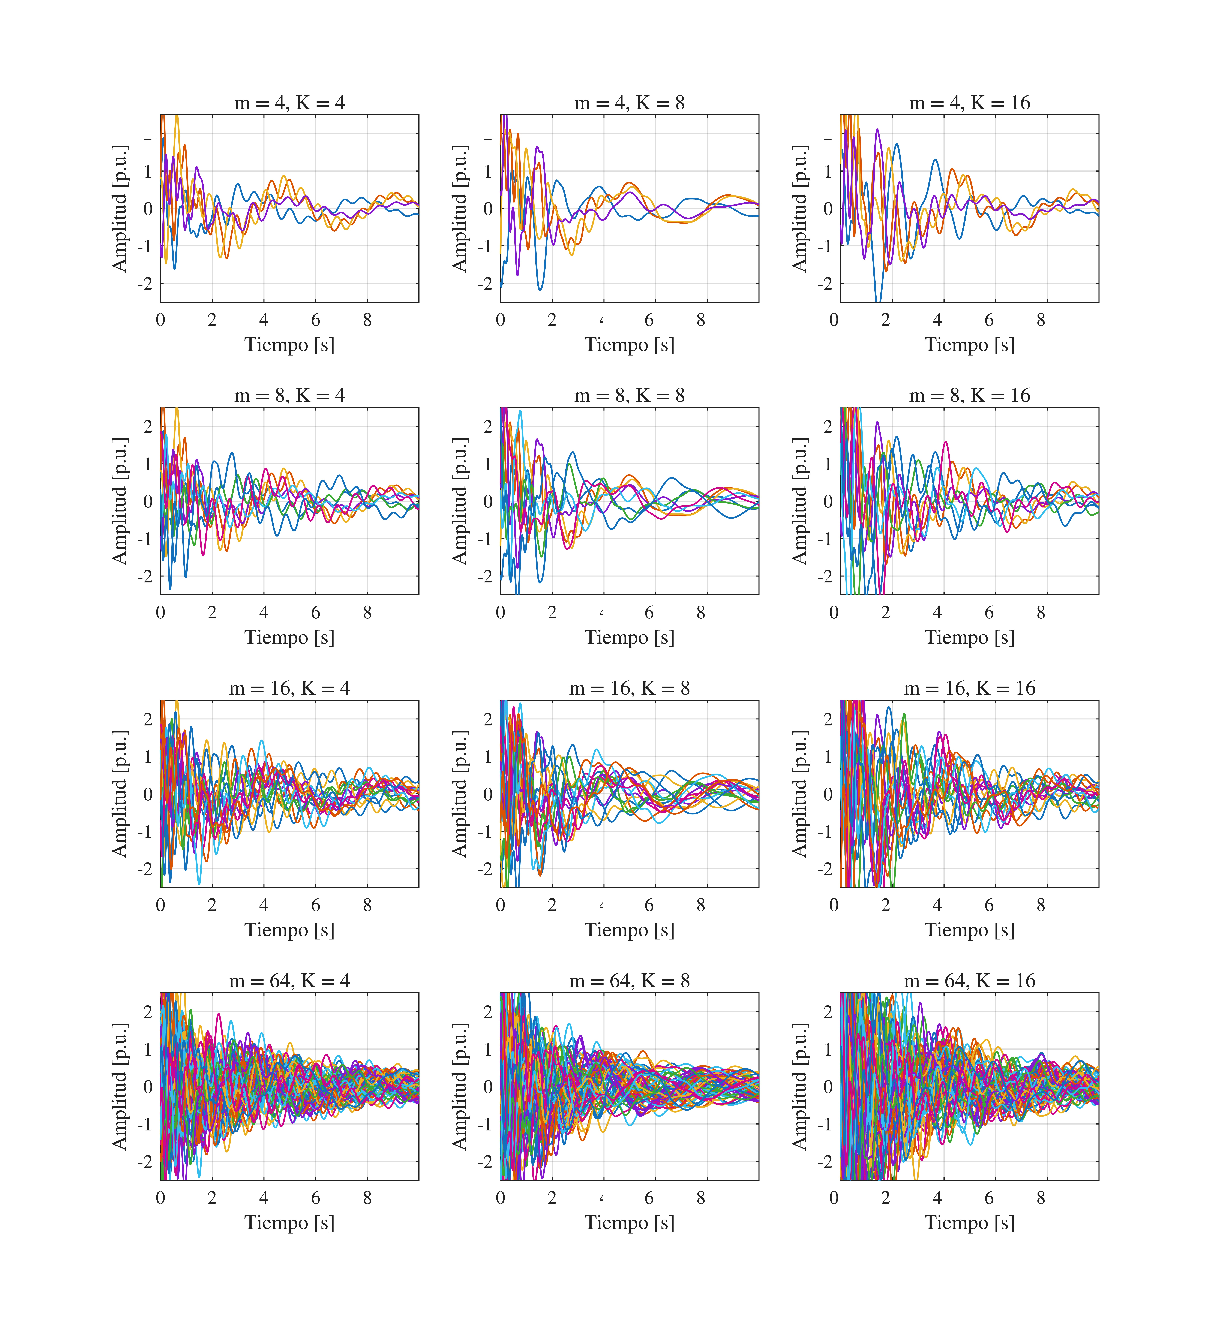
\includegraphics[width=\textwidth]{figuras/Capitulo3/Test.pdf}
    \caption{Señales de prueba sintéticas.}
    \label{fig:signals_test}
\end{figure}

\begin{figure}[t]
    \centering
   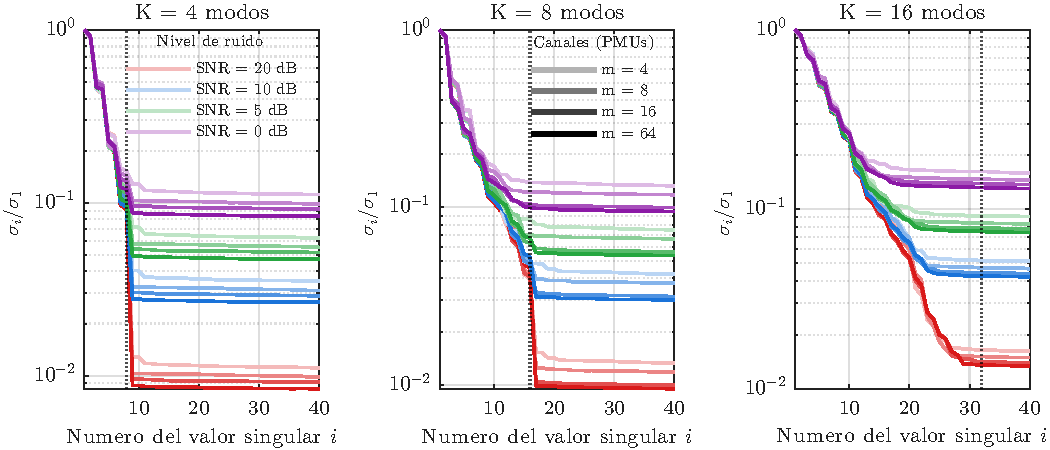
\includegraphics[width=\textwidth]{figuras/Capitulo3/Distribucion_eigenvalues.pdf}
    \caption{Distribución de los valores propios de las señales de prueba.}
    \label{fig:distribution_eigenvalues}
\end{figure}

\begin{figure}[t]
    \centering
    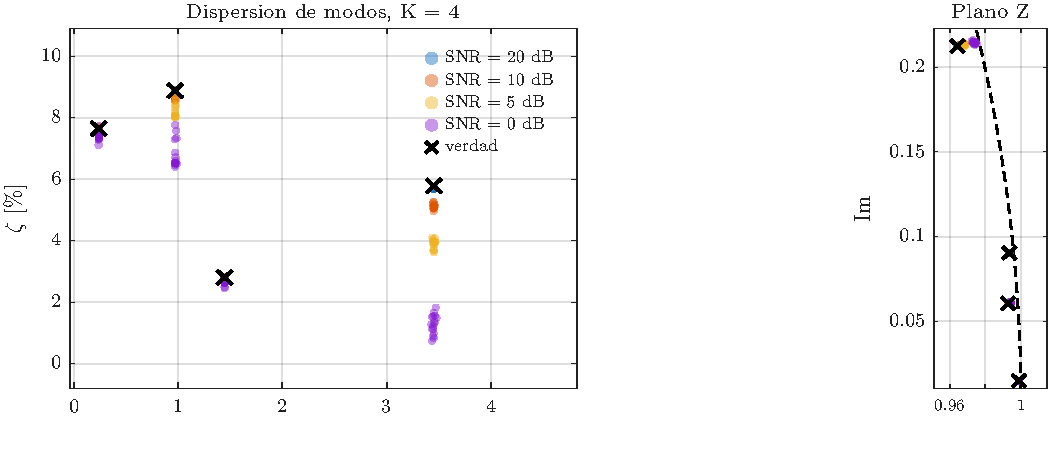
\includegraphics[width=\textwidth]{figuras/Capitulo3/PlanoZ_k_4.pdf}
        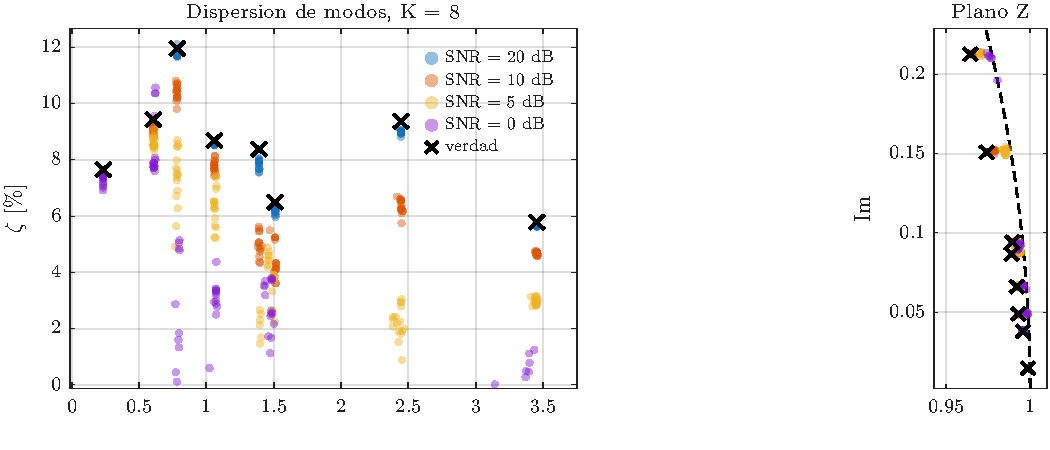
\includegraphics[width=\textwidth]{figuras/Capitulo3/PlanoZ_k_8.pdf}
    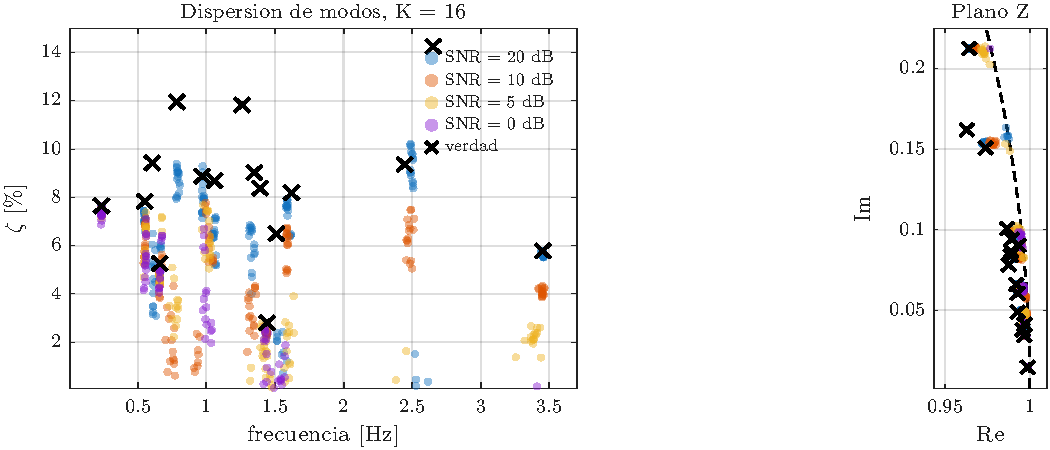
\includegraphics[width=\textwidth]{figuras/Capitulo3/PlanoZ_k_16.pdf}

    \caption{Plano Z de los valores propios de las señales de prueba.}
    \label{fig:Zplane_k_4}
\end{figure}